\documentclass[ignorenonframetext,]{beamer}
\setbeamertemplate{caption}[numbered]
\setbeamertemplate{caption label separator}{: }
\setbeamercolor{caption name}{fg=normal text.fg}
\beamertemplatenavigationsymbolsempty
\usepackage{lmodern}
\usepackage{amssymb,amsmath}
\usepackage{ifxetex,ifluatex}
\usepackage{fixltx2e} % provides \textsubscript
\ifnum 0\ifxetex 1\fi\ifluatex 1\fi=0 % if pdftex
  \usepackage[T1]{fontenc}
  \usepackage[utf8]{inputenc}
\else % if luatex or xelatex
  \ifxetex
    \usepackage{mathspec}
  \else
    \usepackage{fontspec}
  \fi
  \defaultfontfeatures{Ligatures=TeX,Scale=MatchLowercase}
\fi
\usetheme[]{Montpellier}
\usecolortheme{dolphin}
\usefonttheme{structurebold}
% use upquote if available, for straight quotes in verbatim environments
\IfFileExists{upquote.sty}{\usepackage{upquote}}{}
% use microtype if available
\IfFileExists{microtype.sty}{%
\usepackage{microtype}
\UseMicrotypeSet[protrusion]{basicmath} % disable protrusion for tt fonts
}{}
\newif\ifbibliography
\hypersetup{
            pdftitle={Module 3 - Analyse statistique avec R - Séance 2 : PCA et PCoA},
            pdfauthor={Magali Berland},
            pdfborder={0 0 0},
            breaklinks=true}
\urlstyle{same}  % don't use monospace font for urls

% Prevent slide breaks in the middle of a paragraph:
\widowpenalties 1 10000
\raggedbottom

\AtBeginPart{
  \let\insertpartnumber\relax
  \let\partname\relax
  \frame{\partpage}
}
\AtBeginSection{
  \ifbibliography
  \else
    \let\insertsectionnumber\relax
    \let\sectionname\relax
    \frame{\sectionpage}
  \fi
}
\AtBeginSubsection{
  \let\insertsubsectionnumber\relax
  \let\subsectionname\relax
  \frame{\subsectionpage}
}

\setlength{\parindent}{0pt}
\setlength{\parskip}{6pt plus 2pt minus 1pt}
\setlength{\emergencystretch}{3em}  % prevent overfull lines
\providecommand{\tightlist}{%
  \setlength{\itemsep}{0pt}\setlength{\parskip}{0pt}}
\setcounter{secnumdepth}{0}

\title{Module 3 - Analyse statistique avec R - Séance 2 : PCA et PCoA}
\subtitle{DUBii 2019}
\author{Magali Berland}
\date{2019-02-01}

\begin{document}
\frame{\titlepage}

\begin{frame}
\tableofcontents[hideallsubsections]
\end{frame}

\begin{frame}{Analyse en Composantes principales}

Objectif : décrire sans a priori un tableau de données constitué
exclusivement de variables quantitatives.

\begin{center}\includegraphics[width=400px]{figures/07_tests_multiplesunnamed-chunk-2-1} \end{center}

\end{frame}

\begin{frame}{Analyse en Composantes principales}

\begin{center}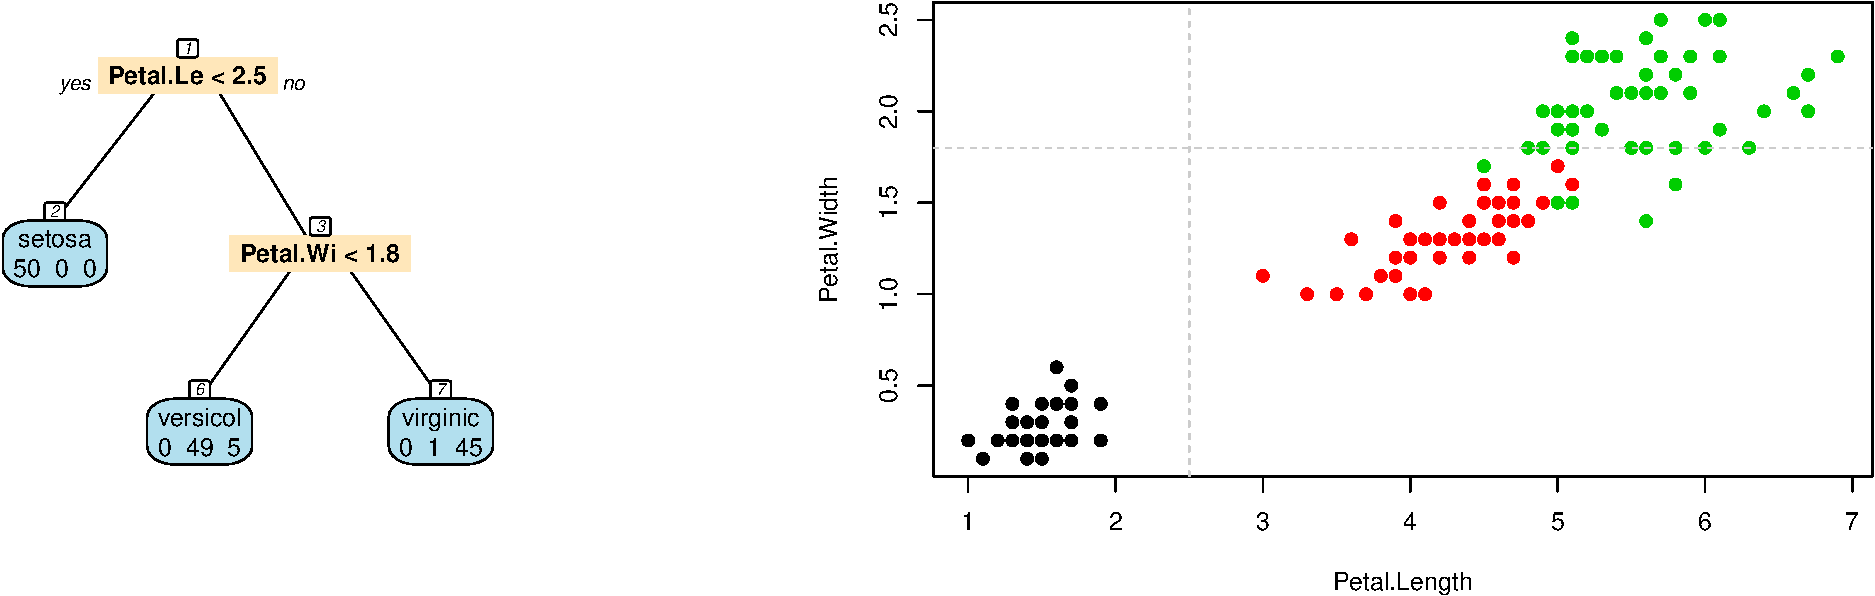
\includegraphics[width=600px]{figures/07_tests_multiplesunnamed-chunk-3-1} \end{center}

\end{frame}

\begin{frame}{Analyse en Composantes principales}

L'ACP permet de déterminer :

\begin{itemize}
\tightlist
\item
  les espaces de dimension inférieure à l'espace initial
\item
  sur lesquels la projection du nuage de points initial est la moins
  déformée possible,
\item
  celle qui conserve le plus d'information c'est-à-dire de variabilité.
\end{itemize}

\end{frame}

\begin{frame}{Analyse en Composantes principales}

Le principe de l'ACP :

\begin{itemize}
\tightlist
\item
  Trouver un axe ( = la première composante principale),
\item
  Issu d'une combinaison linéaire des variables initiales,
\item
  Tel que la variance du nuage autour de cet axe soit maximale.
\item
  Réitérer ce processus dans des directions orthogonales pour déterminer
  les composantes principales suivantes.
\end{itemize}

\end{frame}

\begin{frame}{Analyse en Composantes principales}

\begin{itemize}
\item
  l'ACP permet de conserver au mieux la structure de corrélation entre
  les variables initiales.
\item
  Plusieurs variables corrélées :
\item
  Première composante principale = combinaison de ces variables
\item
  Suffit à représenter les individus avec une perte d'information
  minimale
\item
  Tous les points sont relativement proches de ce nouvel axe.
\end{itemize}

\end{frame}

\begin{frame}{Notions de base}

\begin{center}\includegraphics[width=500px]{figures/07_tests_multiplesunnamed-chunk-4-1} \end{center}

\begin{itemize}
\tightlist
\item
  L'ACP suppose que les directions avec les plus grandes variances sont
  les plus ``importantes''
\item
  La quantité de variance expliquée par chaque composante principale est
  mesurée par ce que l'on appelle valeur propre.
\item
  L'ACP est particulièrement utile lorsque les variables sont fortement
  corrélées (réduction de dimension)
\end{itemize}

\end{frame}

\begin{frame}{Standardisation des données}

\begin{itemize}
\tightlist
\item
  Pour faire une ACP, les variables sont souvent normalisées
\item
  Particulièrement recommandé lorsque les variables sont mesurées dans
  différentes unités
\item
  L'objectif est de rendre les variables comparables.
\end{itemize}

\end{frame}

\begin{frame}{Standardisation des données}

\begin{itemize}
\tightlist
\item
  Pour faire une ACP, les variables sont souvent normalisées
\item
  Particulièrement recommandé lorsque les variables sont mesurées dans
  différentes unités
\item
  L'objectif est de rendre les variables comparables.
\item
  Centrer et réduire = soustraire à chaque valeur la moyenne de la
  variable et diviser par l'écart-type : \#insert formula
\item
  L'ACP appliquée à ces données transformées est appelée ACP normée.
\item
  La fonction scale() peut être utilisée pour normaliser les données.
\end{itemize}

\end{frame}

\end{document}
